\begin{chapter}{Validation and Benchmarking}

For all new computer programs, an important step in the development
process is the validation of the program against other computational
tools.  In the field of fusion activation calculations, there are many
such tools.  Both FISPACT-97 and DKR have been shown in the past to
agree well with analytical solutions to multi-step activation
pathways\cite{IAEA.bench2.rep}.  \ALARA\ offers improvement over
DKR because it is able to accurately model loops in the activation
trees and calculate the gas production.  In comparison to FISPACT-97,
\ALARA\ has many advantages, including the ability to exactly model
pulsed irradiation histories and simultaneously calculate the solution
at many spatial points.  In comparison to both codes, \ALARA\ uses
modern programming practices and data handling to increase the
flexibility of operation and reduce memory requirements.

\section{Benchmark Specifications}

The IAEA FENDL Calculational Activation
Benchmark\cite{IAEA.bench1.spec} problem is based on the reference
steel/water shielding blanket design in the ITER outline design shown
in figure \ref{fig:valid.radial_build}.  This design includes:
\begin{itemize}
\item a copper first wall with beryllium coating
\item shielding blanket with alternating layers of stainless steel
  (316 SS) and water
\item a double wall Inconel 625 vacuum vessel with a water-cooled
  steel pebble bed and a back shield made of lead and boron carbide
\item an inboard magnet, including conductors and insulators.
\end{itemize}
With such a wide range of materials, the design offers an extensive
test of the activation code's capabilities.

The neutron fluxes have been provided by the benchmark in the
VITAMIN-J 175 group energy structure for each of the 468 fine mesh
intervals.  These fluxes were calculated using the
ONEDANT\cite{ONEDANT} deterministic neutron transport code with a
14.1 MeV isotropic neutron source normalized to inboard and outboard
neutron wall loadings of 1 and 1.5 MW/m$^2$, respectively.

Version 2.0 of the IAEA Fusion Evaluated Nuclear Data Library for
Activation (FENDL/A 2.0) and for Decay (FENDL/D 2.0) were used for all
calculations, ensuring that difference in the results were due to the
activation codes themselves and not the nuclear data.

The first activation calculations were performed with a steady state
operation time of 3 years and cooling times of 1 hour, 1 day, 1 week,
30 days, 1 year and 100 years.  A pulsed activation calculation was
performed by \ALARA\ and DKR using 94500 pulses of 1000 s with a dwell
time of 1200 s between pulses.\footnote{Based on the time (14 minutes)
  required to solve the first 100 pulses at a single spatial point,
  FISPACT-97 was determined to be unsuited to such pulsed operation
  calculations.  Assuming that the total operation time scales
  linearly with the number of pulses, the full problem would require
  more than 220 days for each of the 317 spatial points -- a total
  computation time of over 190 years!}

\section{Steady-State Problem}

In \ALARA\, this calculation built 111 reaction trees with a total of
45075 nodes and a longest chain of length 14, producing 770 different
isotopes in the steel-containing intervals, of which 550 were
radioactive.

The results have been compared by calculating the relative difference
between \ALARA\ and the other codes:
$$\mbox{Relative Difference} = \frac{\mbox{\ALARA}}{\mbox{X}} - 1,$$
where X is either FISPACT-97 or DKR.  

\begin{figure}[htbp]
  \begin{center}
%    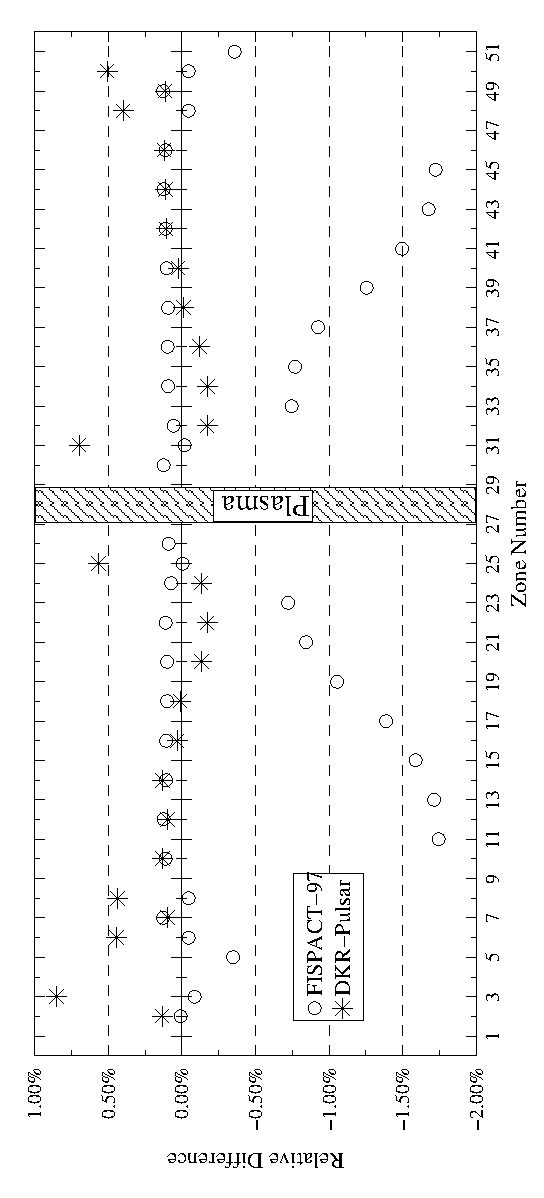
\epsfig{file=eps/1h_final.eps,height=\textwidth,angle=-90}
    \caption{Relative difference between ALARA and other codes for
      steady state problem at a cooling time of 1 hour.}
    \label{fig:rel.diff.ss.1}
  \end{center}
\end{figure}

\begin{figure}[htbp]
  \begin{center}
%    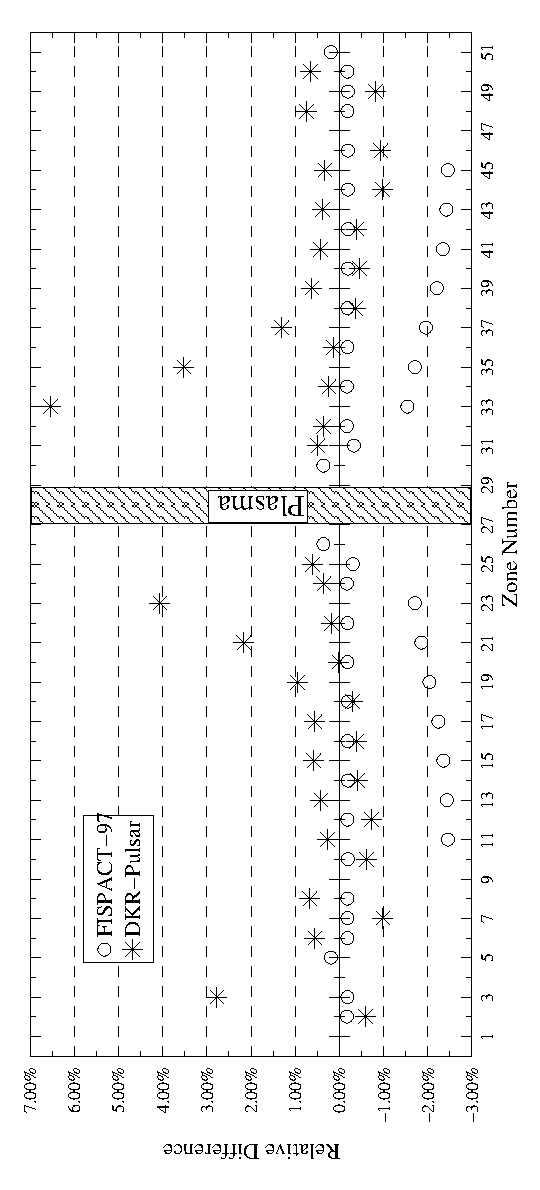
\epsfig{file=eps/1c_final.eps,height=\textwidth,angle=-90}
    \caption{Relative difference between \ALARA\ and other codes for
      steady state problem at a cooling time of 1 century.}
    \label{fig:rel.diff.ss.2}
  \end{center}
\end{figure}

Figures \ref{fig:rel.diff.ss.1} and \ref{fig:rel.diff.ss.2} show the
relative difference between the results of the steady state problem
from \ALARA\ and FISPACT-97 and between \ALARA\ and DKR at a cooling time
of 1 hour and 1 century, respectively.  Since the methods implemented
in this version of DKR were not designed to compute the accumulation of
light ions ($^1$H, $^2$H, $^3$H, $^3$He, and $^4$He) emitted by
nuclear reactions, its total activity for all zones with dominant
tritium inventories is much too small.  Since these differences were
up to a few orders of magnitude, the relative difference between \ALARA\
and DKR in these zones has not been shown in figure
\ref{fig:rel.diff.ss.1} in order to compare the differences in the
other zones.

At a cooling time of 1 hour, the \ALARA\ results are within 1.8\% of the
FISPACT-97 results throughout the entire geometry, with most zones
having a difference of less than 0.4\%.  The largest differences occur
in the 14 water-filled zones of the blanket, increasing in directions
away from the plasma in the zones with lower and softer fluxes.  The
absolute activity in these regions is as low as 2.1 $\times$ 10$^9$
Bq/m$^3$ (zone \#11) and dominated by very low levels of tritium (5.4
tritium atoms per 10$^{12}$ source atoms) and $^{14}$C (2.8 atoms per
10$^9$ source atoms).  This demonstrates a difference in the precision
of the two calculations and the way that this precision is defined.
In this case, the \ALARA\ calculation had a precision defined directly
as 1 atom per 10$^{10}$ source atoms whereas FISPACT-97 calculated
inventories as low as 10$^{5}$ atoms corresponding to 1 atom per
10$^{18}$ source atoms in water.  At a cooling time of 1 century, the
differences between \ALARA\ and FISPACT-97 are as high as 2.5\%, with
the largest differences still occurring in the water-filled zones
where, after more than 8 tritium half-lives, the dominant isotope is
now $^{14}$C.  The differences in the other zones remain below 0.4\%.

In those zones with insignificant tritium inventories, the differences
between \ALARA\ and DKR are less than 0.2\% throughout the geometry at a
cooling time of 1 hour.  After 1 century, although the relative
contribution of tritium has increased in some of those same zones, the
relative differences are still less than 1\%.  DKR's inability to
account for the light ion production results in tritium inventories
which are as much as 6 orders of magnitude too low in the first wall's
Be coating, and up to 3 times too low in the blanket's water cooling
zones.  Even after more than 8 tritium half-lives (1
century), when tritium is responsible for less than 10\% of the total
activity, the difference between \ALARA\ and DKR in the water can be as
high as 7\% (zone \#33).

\begin{table}[b]
  \begin{center}
    \caption{Detailed differences in interval \#242 at 1 hour.}
    \label{tab:detail.1}
    \begin{tabular}{|c|c|c|c|}
      \hline
      Isotope & \ALARA\ & \multicolumn{2}{c|}{Relative Difference [\%]} \\
              & [10$^{16}$Bq/m$^3$] & FISPACT-97 & DKR-Pulsar 2.0\\\hline
      $^{56}$Mn & 114.6 & -0.051 & 0.15 \\\hline
      $^{55}$Fe & 85.5 & 0.24 & -0.10 \\\hline
      $^{51}$Cr & 75.7 & 0.019 & -0.041 \\\hline
      $^{57}$Co & 24.4 & -0.081 &  3.0  \\\hline
      $^{54}$Mn & 20.0 & 0.97  &  0.15 \\\hline
      $^{58m}$Co & 10.3 & -0.053 & 0.30 \\\hline
      $^{58}$Co & 8.32 & -0.048 & -13.74  \\\hline
    \end{tabular}
  \end{center}
\end{table}

A single fine mesh interval was chosen in which to compare the
activity of various nuclides in detail.  The 1 mm thick stainless steel
(SS316) inboard first wall back plate is modeled as a single interval
(\#242) in zone \#24.  The large number of initial isotopes in steel
and the high flux due to its proximity to the plasma make this a good
choice for comparison.

Table \ref{tab:detail.1} shows the seven most dominant isotopes at a
cooling time of 1 hour, which together account for over 95\% of the
total activity.  Table \ref{tab:detail.2} shows the five most dominant
isotopes at a cooling time of 1 century, accounting for more than 99.7\% of
the total activity.  

\begin{table}[b]
  \begin{center}
    \caption{Detailed differences in interval \#242 at 1 century.}
    \label{tab:detail.2}
    \begin{tabular}{|c|c|c|c|}
      \hline
      Isotope & \ALARA\ & \multicolumn{2}{c|}{Relative Difference [\%]} \\
              & [10$^{13}$Bq/m$^3$] & FISPACT-97 & DKR-Pulsar 2.0\\\hline
      $^{63}$Ni & 27.8 & -0.17 &  0.40 \\\hline
      $^{59}$Ni & 3.80 & -0.18  & -1.2 \\\hline
      $^{91}$Nb & 3.37 & -0.21  &  1.3  \\\hline
      $^{14}$C  & 0.86 & -0.22  & -0.19 \\\hline
      $^{93}$Mo & 0.69 & -0.21  & 16   \\\hline
    \end{tabular}
  \end{center}
\end{table}

The agreement between \ALARA\ and FISPACT-97 is seen to be within 1\% in
all cases.  DKR, on the other hand, has relative differences of up to
16\%.  These discrepancies are most probably caused by the inability
of DKR to model certain kinds of loops in the decay chains and the
influence which this has on the decay chain creation calculations.

\section{Pulsing Problem}

\begin{figure}[htbp]
  \begin{center}
%    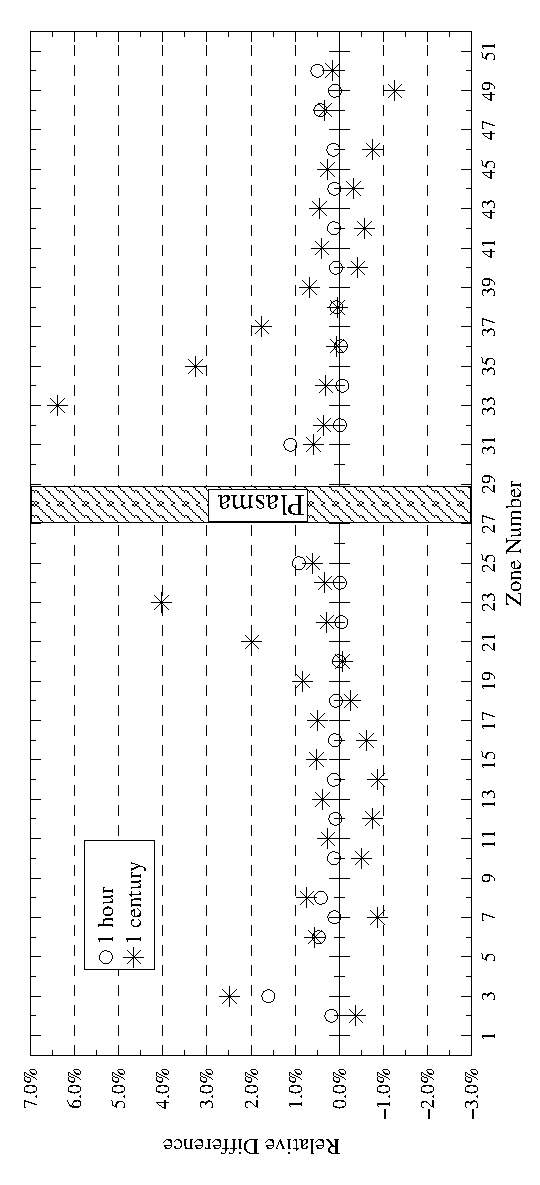
\epsfig{file=eps/pulse_final.eps,height=\textwidth,angle=-90}
    \caption{Relative difference between \ALARA\ and DKR for
      the pulsing problem at cooling times of 1 hour and 1 century.}
    \label{fig:rel.diff.p.1}
  \end{center}
\end{figure}

\begin{figure}[htbp]
  \begin{center}
%    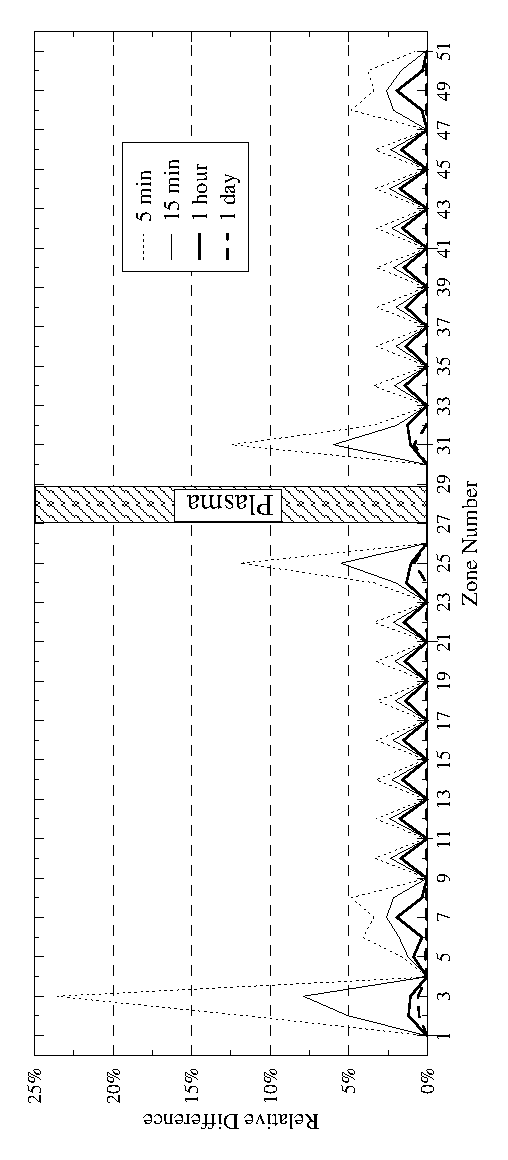
\epsfig{file=eps/ss_approx_final.eps,height=\textwidth,angle=-90}
    \caption{Relative difference between exact pulsed solution and steady state approximation at various cooling times.}
    \label{fig:rel.diff.approx}
  \end{center}
\end{figure}
The results of \ALARA\ and DKR for the pulsing problem are compared in
Figure \ref{fig:rel.diff.p.1} for both 1 hour and 1 century.  Once
again, tritium plays an important role in the discrepancies, which are
nearly identical to the discrepancies between \ALARA\ and DKR for the
steady state problem.  In the glass insulator of the TF coil (zone
\#3), the discrepancy in the pulsing problem is twice as high as in
the steady state problem at 1 hour, but the same at 1 century.  This
demonstrates the true physical effect of pulsing on the importance of
the tritium inventory at relatively short cooling times.  Basically,
the pulsed operation will tend to reduce the inventory of isotopes
with half-lives which are of the same order of magnitude as the dwell
time between pulses: very long-lived isotopes will decay little
between pulses and slowly reach their saturation level while very
short-lived isotopes will decay completely between pulses, but can
reach their saturation level in a single pulse\cite{sisolak}.  The
dominant isotopes in the glass at 1 hour are $^{64}$Cu and $^{24}$Na,
both with half-lives slightly longer than half a day.  Their
inventories in the pulsed problem are 50\% less than in the steady
state problem, while the tritium inventory is reduced by less than
10\%.

One method of modeling a pulsed problem as a steady state problem is
to preserve both the total fluence and the total operating
time\cite{sisolak,hosny,qingming}.  Using ALARA, the
results of such an approximate calculation with a flux scaling factor
of 1/2.2 and total operation time of 2.079 $\times$ 10$^8$ are
compared to the exact solution in Figure \ref{fig:rel.diff.approx},
represented as
$$\mbox{Relative Difference} = \frac{\mbox{Pulsing}}{\mbox{Steady
    State}} - 1.$$
In this case, because of the nature of the pulsing history, the effect
can only be seen at short cooling times.  The two materials with
largest discrepancies are the glass insulator (zone \#3) and the first
wall heat sink (Cu-Be-Ni in zones \#25 and \#31).  In the former, the
activity of $^{28}$Al (t$_{1/2}$ = 2.25 m), responsible for over 25\%
of the activity at a cooling time of 1 minute, is under-calculated by
50\%.  The same is true of $^{66}$Cu (t$_{1/2}$ = 5.10 m) which is
responsible for just under 10\% of the activity in the first wall.
    


\section{Computing Resources}

All three codes were used on the same IBM RS/6000 Model 595 P2SC
workstation.  The full steady-state problem was solved by \ALARA\ in
3425 s (57$^m$5$^s$) and by DKR in 5253 s (1$^h$27$^m$33$^s$).  The
same problem required 20715 s (5$^h$36$^m$25$^s$) for a previously
developed shell-script system which sequentially runs FISPACT-97 for
each of the intervals.  The pulsed problem was solved by \ALARA\ in 5736
s (1$^h$35$^m$36$^s$), with 44591 nodes and a longest chain of 14.
DKR needed 10855 s (3$^h$0$^m$55$^s$).  FISPACT-97 was unable to solve
the pulsed problem.

For the steady state problem, \ALARA\ requires a maximum of 35 MB of RAM
and, other than the binary library of just over 11 MB, uses no hard
drive space.  DKR required as much as 107 MB of RAM and up to
250 MB of temporary hard drive space in addition to its 10 MB text
library.  Other than the 38 MB data libraries, FISPACT-97 uses
negligible quantities of RAM and hard drive space since it solves each
interval sequentially.


\section{Conclusions}

The \ALARA\ activation code has been validated for use in calculating
the activation of fusion power systems.  The results for a steady
state activation problem have been compared to the results from two
standard codes whose accuracy has been well
documented\cite{IAEA.bench2.rep}: FISPACT-97 and DKR.
Discrepancies between the total activities calculated by \ALARA\ and the
other codes are always less than 2.5\%, except where DKR is
unable to calculate the tritium production from emitted light ions.
The results of a pulsing problem have been compared to DKR
(FISPACT-97 was unable to perform such a calculation in a reasonable
time).  The discrepancies in this case are once again primarily due to
the lack of tritium production in DKR, and are otherwise less
than 1\%.

Based on this validation and its faster and less memory-intensive
operation, \ALARA\ is recommended for the solution of fusion activation
problems.


\end{chapter}